\documentclass{report}
\usepackage{graphicx, tikz-cd, float, titlepic, booktabs} % Required for inserting images
\usepackage{pgfplots}
\pgfplotsset{compat=1.15}
\usepackage{mathrsfs}
\usetikzlibrary{arrows}
\usepackage{amsmath, amssymb, amsthm, amsfonts, siunitx, physics, gensymb}
\AtBeginDocument{\RenewCommandCopy\qty\SI}
\usepackage[version=4]{mhchem}
\usepackage[most,many,breakable]{tcolorbox}
\usepackage{xcolor, fancyhdr, varwidth}
\usepackage[Glenn]{fncychap}
%Options: Sonny, Lenny, Glenn, Conny, Rejne, Bjarne, Bjornstrup
\usepackage{hyperref, cleveref}
\usepackage{icomma, enumitem} %comma as decimal and continue enumerate with [resume]
\usepackage{plimsoll} %use standard state symbol with \stst
\usepackage[danish]{babel}
%%%%%%%%%%%%%%%%%%%%%%%%%%%%%%
% SELF MADE COLORS
%%%%%%%%%%%%%%%%%%%%%%%%%%%%%%
\definecolor{myg}{RGB}{56, 140, 70}
\definecolor{myb}{RGB}{45, 111, 177}
\definecolor{myr}{RGB}{199, 68, 64}
\definecolor{mytheorembg}{HTML}{F2F2F9}
\definecolor{mytheoremfr}{HTML}{00007B}
\definecolor{mylenmabg}{HTML}{FFFAF8}
\definecolor{mylenmafr}{HTML}{983b0f}
\definecolor{mypropbg}{HTML}{f2fbfc}
\definecolor{mypropfr}{HTML}{191971}
\definecolor{myexamplebg}{HTML}{F2FBF8}
\definecolor{myexamplefr}{HTML}{88D6D1}
\definecolor{myexampleti}{HTML}{2A7F7F}
\definecolor{mydefinitbg}{HTML}{E5E5FF}
\definecolor{mydefinitfr}{HTML}{3F3FA3}
\definecolor{notesgreen}{RGB}{0,162,0}
\definecolor{myp}{RGB}{197, 92, 212}
\definecolor{mygr}{HTML}{2C3338}
\definecolor{myred}{RGB}{127,0,0}
\definecolor{myyellow}{RGB}{169,121,69}
\definecolor{myexercisebg}{HTML}{F2FBF8}
\definecolor{myexercisefg}{HTML}{88D6D1}
%%%%%%%%%%%%%%%%%%%%%%%%%%%%%%%%%%%%%%%%%%%%%%%%%%%%%%%%%%%%%%%%%%%%%%
% Box environments for theorems and problems
%%%%%%%%%%%%%%%%%%%%%%%%%%%%%%%%%%%%%%%%%%%%%%%%%%%%%%%%%%%%%%%%%%%%%
\setlength{\parindent}{1cm}
%================================
% Question BOX
%================================
\makeatletter
\newtcbtheorem{question}{Opgave}{enhanced,
	breakable,
	colback=white,
	colframe=myb!80!black,
	attach boxed title to top left={yshift*=-\tcboxedtitleheight},
	fonttitle=\bfseries,
	title={#2},
	boxed title size=title,
	boxed title style={%
			sharp corners,
			rounded corners=northwest,
			colback=tcbcolframe,
			boxrule=0pt,
		},
	underlay boxed title={%
			\path[fill=tcbcolframe] (title.south west)--(title.south east)
			to[out=0, in=180] ([xshift=5mm]title.east)--
			(title.center-|frame.east)
			[rounded corners=\kvtcb@arc] |-
			(frame.north) -| cycle;
		},
	#1
}{def}
\makeatother
%================================
% DEFINITION BOX
%================================

\newtcbtheorem[]{Definition}{Definition}{enhanced,
	before skip=2mm,after skip=2mm, colback=red!5,colframe=red!80!black,boxrule=0.5mm,
	attach boxed title to top left={xshift=1cm,yshift*=1mm-\tcboxedtitleheight}, varwidth boxed title*=-3cm,
	boxed title style={frame code={
					\path[fill=tcbcolback]
					([yshift=-1mm,xshift=-1mm]frame.north west)
					arc[start angle=0,end angle=180,radius=1mm]
					([yshift=-1mm,xshift=1mm]frame.north east)
					arc[start angle=180,end angle=0,radius=1mm];
					\path[left color=tcbcolback!60!black,right color=tcbcolback!60!black,
						middle color=tcbcolback!80!black]
					([xshift=-2mm]frame.north west) -- ([xshift=2mm]frame.north east)
					[rounded corners=1mm]-- ([xshift=1mm,yshift=-1mm]frame.north east)
					-- (frame.south east) -- (frame.south west)
					-- ([xshift=-1mm,yshift=-1mm]frame.north west)
					[sharp corners]-- cycle;
				},interior engine=empty,
		},
	fonttitle=\bfseries,
	title={#2},#1}{def}
\newtcbtheorem[]{definition}{Definition}{enhanced,
	before skip=2mm,after skip=2mm, colback=red!5,colframe=red!80!black,boxrule=0.5mm,
	attach boxed title to top left={xshift=1cm,yshift*=1mm-\tcboxedtitleheight}, varwidth boxed title*=-3cm,
	boxed title style={frame code={
					\path[fill=tcbcolback]
					([yshift=-1mm,xshift=-1mm]frame.north west)
					arc[start angle=0,end angle=180,radius=1mm]
					([yshift=-1mm,xshift=1mm]frame.north east)
					arc[start angle=180,end angle=0,radius=1mm];
					\path[left color=tcbcolback!60!black,right color=tcbcolback!60!black,
						middle color=tcbcolback!80!black]
					([xshift=-2mm]frame.north west) -- ([xshift=2mm]frame.north east)
					[rounded corners=1mm]-- ([xshift=1mm,yshift=-1mm]frame.north east)
					-- (frame.south east) -- (frame.south west)
					-- ([xshift=-1mm,yshift=-1mm]frame.north west)
					[sharp corners]-- cycle;
				},interior engine=empty,
		},
	fonttitle=\bfseries,
	title={#2},#1}{def}

\newtcbtheorem{theo}%
    {Theorem}{}{theorem}
\newtcolorbox{prob}[1]{colback=red!5!white,colframe=red!50!black,fonttitle=\bfseries,title={#1}}
%================================
% NOTE BOX
%================================

\usetikzlibrary{arrows,calc,shadows.blur}
\tcbuselibrary{skins}
\newtcolorbox{note}[1][]{%
	enhanced jigsaw,
	colback=gray!20!white,%
	colframe=gray!80!black,
	size=small,
	boxrule=1pt,
	title=\textbf{Note:},
	halign title=flush center,
	coltitle=black,
	breakable,
	drop shadow=black!50!white,
	attach boxed title to top left={xshift=1cm,yshift=-\tcboxedtitleheight/2,yshifttext=-\tcboxedtitleheight/2},
	minipage boxed title=1.5cm,
	boxed title style={%
			colback=white,
			size=fbox,
			boxrule=1pt,
			boxsep=2pt,
			underlay={%
					\coordinate (dotA) at ($(interior.west) + (-0.5pt,0)$);
					\coordinate (dotB) at ($(interior.east) + (0.5pt,0)$);
					\begin{scope}
						\clip (interior.north west) rectangle ([xshift=3ex]interior.east);
						\filldraw [white, blur shadow={shadow opacity=60, shadow yshift=-.75ex}, rounded corners=2pt] (interior.north west) rectangle (interior.south east);
					\end{scope}
					\begin{scope}[gray!80!black]
						\fill (dotA) circle (2pt);
						\fill (dotB) circle (2pt);
					\end{scope}
				},
		},
	#1,
}
%================================
% EXAMPLE BOX
%================================
\newtcbtheorem[number within=section]{Example}{Example}
{%
	colback = myexamplebg
	,breakable
	,colframe = myexamplefr
	,coltitle = myexampleti
	,boxrule = 1pt
	,sharp corners
	,detach title
	,before upper=\tcbtitle\par\smallskip
	,fonttitle = \bfseries
	,description font = \mdseries
	,separator sign none
	,description delimiters parenthesis
}
{ex}
%================================
% THEOREM BOX
%================================

\tcbuselibrary{theorems,skins,hooks}
\newtcbtheorem[number within=section]{Theorem}{Theorem}
{%
	enhanced,
	breakable,
	colback = mytheorembg,
	frame hidden,
	boxrule = 0sp,
	borderline west = {2pt}{0pt}{mytheoremfr},
	sharp corners,
	detach title,
	before upper = \tcbtitle\par\smallskip,
	coltitle = mytheoremfr,
	fonttitle = \bfseries\sffamily,
	description font = \mdseries,
	separator sign none,
	segmentation style={solid, mytheoremfr},
}
{th}

%%%%%%%%%%%%%%%%%%%%%%%%%%%%%%%%%%%%%%%%%%%%%%%%%%%%%%%%%%%%%%%%%
% SELF MADE COMMANDS
%%%%%%%%%%%%%%%%%%%%%%%%%%%%%%
\newcommand{\sol}{\setlength{\parindent}{0cm}\textbf{\textit{Løsning:}}\setlength{\parindent}{1cm}}
%%%%%%%%%%%%%%%%%%%%%%%%%%%%%%%%%
\usepackage[tmargin=2cm,rmargin=1in,lmargin=1in,margin=0.85in,bmargin=2cm,footskip=.2in]{geometry}\pagestyle{fancy}
\lhead{Minrui Kevin Zhou 3.b}
\rhead{Opgavesæt 2}

\title{Opgavesæt 2\\
{\Large \textbf{3.b kemi A}}}
\author{Kevin Zhou}
\date{\today}

\begin{document}
\maketitle
\begin{note}
  Databog fysik kemi (2007) er benyttet ved beregningerne.
\end{note}
\section*{Terpenoider}
\sol \\
\textbf{a.}
På \cref{fig:citral} ses alle carbon- og hydrogenatomer anført på formlen for citral.
\begin{figure}[H]
\begin{center}
  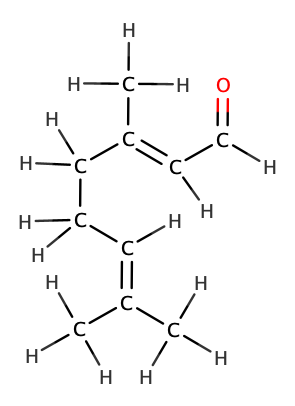
\includegraphics[scale=1.0]{citral.png}
\end{center}
\caption{Carbon- og hydrogenatomer anført på formlen for citral i MarvinSketch}
\label{fig:citral}
\end{figure}
\noindent \textbf{b.}
Det færdiggjorte reaktionsskema ses i \cref{fig:kondensation}.
\begin{figure}[H]
\begin{center}
  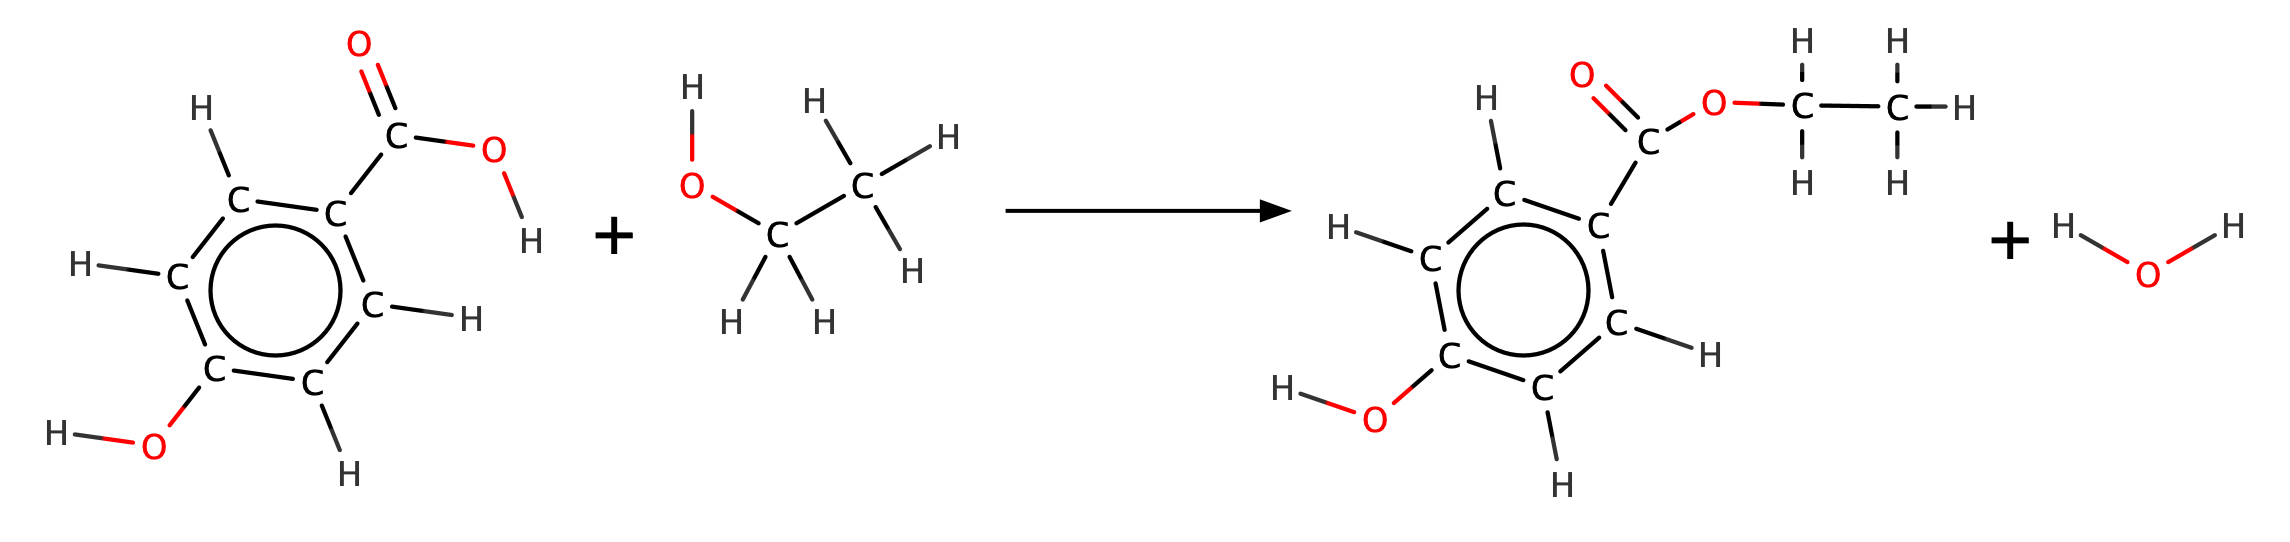
\includegraphics[scale=0.7]{kondensation.png}
\end{center}
\caption{Kondensationsreaktionen tegnet i MarvinSketch}
\label{fig:kondensation}
\end{figure}
\noindent \textbf{c.}
Stoffer, der kan addere dibrom må være umættede.
Et eksempel på en sådan reaktion ses i \cref{fig:dibrom}.
Carbonylforbindelser reagerer med 2,4-dinitrophenylhydrazin og danner gult bundfald i form af hydrazoner.
Aldehyder og ketoner er begge carbonylforbindelser.
For at skelne mellem disse bruger man Tollens reagens eller Fehlings væske.
Disse reagerer begge kun med aldehyder, men ikke ketoner, og giver henholdsvis sølv og rødt bundfald.
Til sidst er det kun muligt for asymmetriske molekyler at dreje polarisationsplanet for planpolariseret lys.
\begin{figure}[H]
\begin{center}
  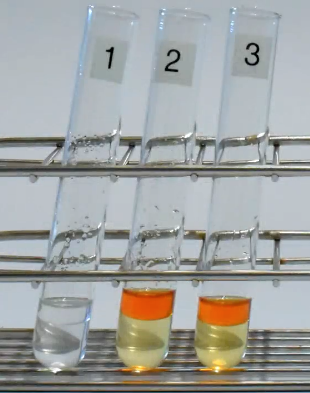
\includegraphics[scale=0.5]{dibrom.png}
\end{center}
\caption{Eksempel på additionsreaktion med dibrom}
\label{fig:dibrom}
\end{figure}
\subsubsection{Glas A}
Da stoffet i glas A reagerer med 2,4-dinitrophenylhydrazin og danner gult bundfald, må stoffet være en carbonylforbindelse.
Stoffet reagerer dog hverken med Fehlings eller Tollens, og må altså være en keton.
Imidlertid ser vi, at menthon er den eneste keton blandt de fem terpenoider.
Altså må menthon være i glas A.
\subsubsection{Glas B}
Stoffet i glas A kan addere dibrom og må være umættet.
Da det ikke reagerer med 2,4-dinitrophenylhydrazin, så må stoffet ikke indholde en carbonylgruppe.
Imidlertid ser vi, at både citral og linalool er umættede (dobbeltbindinger mellem \ce{C}-atomer), men citral indeholder en carbonylgruppe.
Altså må linalool være i glas B.
\subsubsection{Glas C}
Da stoffet i glas C ikke reagerer med 2,4-dinitrophenylhydrazin, så må stoffet ikke indholde en carbonylgruppe.
Linalool, carvacrol og menthol opfylder dette.
Siden linalool er i glas B, så er de eneste muligheder carvacrol og menthol.
Stoffet i glasset kan dog dreje polarisationsplanet for planpolariseret lys og må indholde et assymetrisk \ce{C}-atom, hvilket opfyldes af menthol, men ikke carvacrol.
Altså må menthol være i glas C.
\subsubsection{Glas D}
Stoffet i glas D reagerer med både 2,4-dinitrophenylhydrazin, Tollens samt Fehlings og må derfor være en aldehyd.
Af de fem terpenoider er citral den eneste aldehyd.
Atlså må citral være i glas D.
\subsubsection{Glas E}
Ved brug af udelukkelsesmetoden må carvacrol være i glas E.

\section*{Tilsætningsstoffer i benzin til biler}
\sol \\
\textbf{a.}
Reaktionsskemaet for eliminationsreaktionen, hvor 2-chlor-2-methylpropan omdannes til 2-methylprop-1-en ses i \cref{fig:elimination}.
\begin{figure}[H]
\begin{center}
  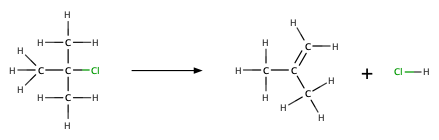
\includegraphics[scale=0.8]{elimination.png}
\end{center}
\caption{Eliminationsreaktionen anført med MarvinSketch}
\label{fig:elimination}
\end{figure}
\noindent \textbf{b.}
Vi sætter de givne data ind i Logger Pro og laver en lineær regression, hvilket ses i \cref{fig:G}.
\begin{figure}[H]
\begin{center}
  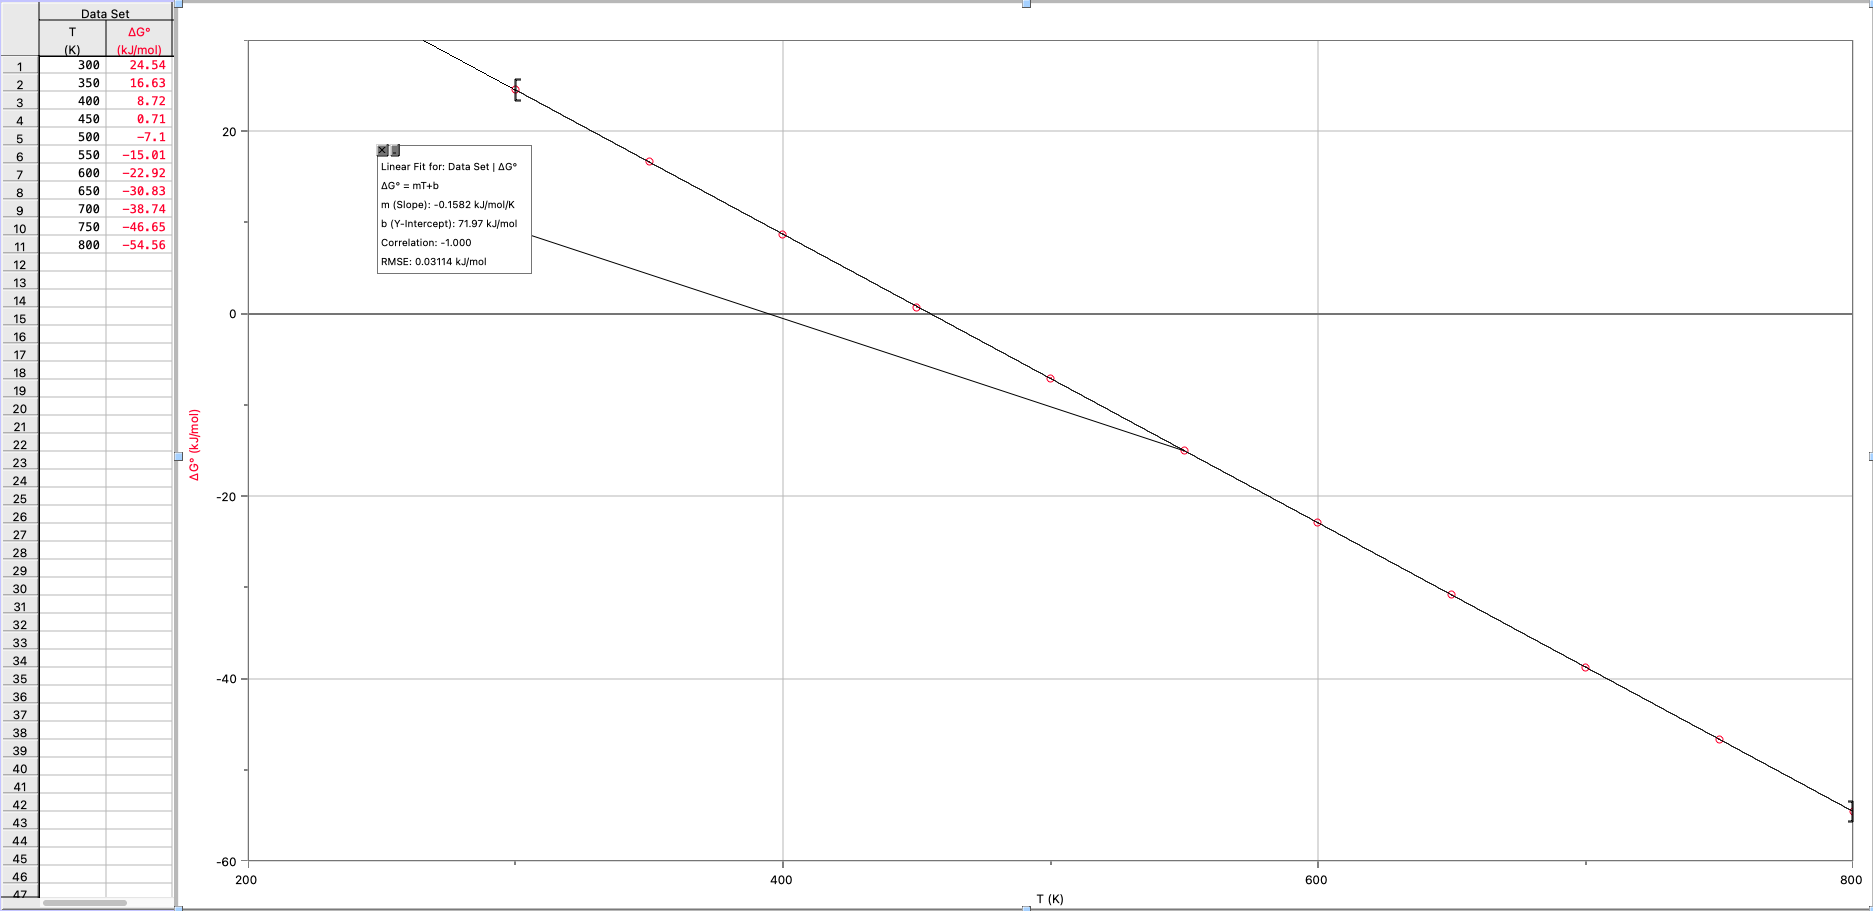
\includegraphics[scale=0.24]{G.png}
\end{center}
\caption{Lineær regression lavet i Logger Pro}
\label{fig:G}
\end{figure}
Fra regressionen har vi
\[
\Delta G \stst =71,97 \;\unit{kJ/mol} -0,1582 \;\unit{\frac{kJ}{mol \cdot K}} \cdot T
\] 
Der gælder for tilvæksten af standard Gibbs-energi, at
\[
\Delta G \stst =\Delta H\stst - \Delta S\stst \cdot T 
\] 
Ved at kombinere de to ligninger får vi, at
\begin{equation*}
\begin{split}
  \Delta H\stst &=71,97 \;\unit{kJ/mol} \\
  &\approx 72 \;\unit{kJ/mol} 
\end{split}
\end{equation*}
Vi får da $\Delta H\stst=72 \;\unit{kJ/mol} >0$, hvilket vil sige, at reaktionen er endoterm ved standardbetingelserne.\\[1ex]
\textbf{c.}
Reaktionen kan forløbe spontant ved standardbetingelserne når 
\begin{equation*}
\begin{split}
  \Delta G \stst <0 &\iff 71,97 \;\unit{kJ/mol} -0,1582 \;\unit{\frac{kJ}{mol \cdot K}} \cdot T <0\\
  &\iff T >\frac{71,97 \;\unit{kJ/mol} }{0,1582 \;\unit{kJ/mol} } \;\unit{K} \approx 4,5 \cdot 10^2 \;\unit{K} 
\end{split}
\end{equation*}
Altså kan reaktionen forløbe, når temperaturen er over $4,5 \cdot 10^2 \;\unit{K} $.\\[1ex]
\textbf{d.}
Vi finder først $\Delta G \stst$ ved $260 \;\unit{\celsius} $. 
\begin{equation*}
\begin{split}
  \Delta G \stst&=71,97 \;\unit{kJ/mol} -0,1582 \;\unit{\frac{kJ}{mol \cdot K}} \cdot T\\
  &=71,97 \;\unit{kJ/mol} -0,1582 \;\unit{\frac{kJ}{mol \cdot K}} \cdot (260 + 273,15) \;\unit{K} \\
  &=-12,37433 \;\unit{kJ/mol} 
\end{split}
\end{equation*}
Siden der indstilles en ligevægt, så gælder der
\begin{equation*}
\begin{split}
  -\Delta G\stst=R \cdot T \cdot \ln\left(K\right) &\iff \ln\left(K\right) = \frac{-\Delta G \stst}{R \cdot T}\\
  &\iff K=e^{\frac{-\Delta G\stst}{R \cdot T}} 
\end{split}
\end{equation*}
Vi beregner nu $K$
\begin{equation*}
\begin{split}
  K&=e^{\frac{-\Delta G\stst}{R \cdot T}} \\
  &=e^{\frac{-(-12,37433 \;\unit{kJ/mol}) }{8,314 \cdot 10^{-3} \;\unit{\frac{kJ}{mol \cdot K}}  \cdot 533,15 \;\unit{K} }} \\
  &=16,308\\
  &\approx 16
\end{split}
\end{equation*}
Ved udregningen får vi ligevægtskonstanten som et ubenævnt tal.
For at finde enheden kam man betragte ligevægtsloven for reaktionen.
\[
K=\frac{p(\text{2-methylprop-1-en})\cdot p(\ce{HCl} )}{p(\text{2-chlor-2-methylpropan})}
\] 
Af brøken ser man, at enheden må være $\unit{bar} $.
Ligevægtskonstanten for reaktionen ved $260 \;\unit{\celsius} $ er altså $16 \;\unit{bar} $.\\[1ex]
\textbf{e.}
Da reaktionsforholdet mellem 2-methylprop-1-en og \ce{HCl} er 1:1, så må der gælde, at
\[
n(\text{2-methylprop-1-en} )=n(\ce{HCl} ) \iff p(\text{2-methylprop-1-en} )=p(\ce{HCl}) 
\] 
Fra ligevægtsloven har vi så, at
\begin{equation*}
\begin{split}
  p(\text{2-chlor-2-methylpropan} )&=\frac{p(\text{2-methylprop-1-en})\cdot p(\ce{HCl} )}{K}\\
  &=\frac{\left(0,52 \;\unit{bar} \right)^2}{16,308 \;\unit{bar} }\\
  &=0,01658 \;\unit{bar} 
\end{split}
\end{equation*}
Vi regner nu stofmængden af 2-chlor-2-methylpropan ud med idealgasloven, da vi kender både partialtrykket, volumen og temperaturen.
\begin{equation*}
\begin{split}
  n(\text{2-chlor-2-methylpropan})&=\frac{p(\text{2-chlor-2-methylpropan}) \cdot V}{R \cdot T}\\
  &=\frac{0,01685 \;\unit{bar} \cdot 3,00 \;\unit{L} }{0,0831 \;\unit{\frac{L \cdot bar}{mol \cdot K}} \cdot 533,15 \;\unit{K} }\\
  &=1,1227 \;\unit{mmol} 
\end{split}
\end{equation*}
Vi kan nu regne massen.
\begin{equation*}
\begin{split}
  m(\text{2-chlor-2-methylpropan} )&=n(\text{2-chlor-2-methylpropan} )\cdot M(\text{2-chlor-2-methylpropan})\\
  &=0,0011227 \;\unit{mol} \cdot 92,57 \;\unit{g/mol} \\
  &\approx 0,10 \;\unit{g} 
\end{split}
\end{equation*}
Massen af 2-chlor-2-methylpropan, der blev anbragt i beholderen fra start er altså $0,10 \;\unit{g} $.

\section*{Flussyre}
\sol \\
\textbf{a.}
Reaktionsskemaet for reaktionen mellem fluorit og svovlsyre må være
\[
\ce{H2SO4 + CaF2 -> 2HF + CaSO4} 
\] 
\textbf{b.}
Vi regner først $pK_s$ for flussyre. 
\begin{equation*}
\begin{split}
  pK_s&=-\log\left(K_s\right) \\
  &=-\log\left(6,76 \cdot 10^{-4}\right) \\
  &=3,170
\end{split}
\end{equation*}
Der gælder da
\begin{equation*}
\begin{split}
K_s=\frac{\left[\ce{H3O+} \right]^2}{c_s-\left[\ce{H3O+} \right]} &\implies \left[\ce{H3O+} \right]=\frac{-K_s + \sqrt{K_s^2 - 4 \cdot \left(-K_s \cdot c_s\right) } }{2}\\
  &\iff pH=- \log\left(\frac{-K_s + \sqrt{K_s^2 - 4 \cdot \left(-K_s \cdot c_s\right) } }{2 \;\unit{\textsc{m}} }\right) 
\end{split}
\end{equation*}
fordi $pH=-\log\left(\frac{[\ce{H3O+} ]}{\unit{\textsc{m}}}\right) $.
Vi indsætter de kendte værdier og udregner pH.
\begin{equation*}
\begin{split}
  pH&=- \log\left(\frac{-K_s + \sqrt{K_s^2 - 4 \cdot \left(-K_s \cdot c_s\right) } }{2 \;\unit{\textsc{m}} }\right) \\
  &=-\log\left(\frac{-6,76 \cdot 10^{-4}\;\unit{\textsc{m}} + \sqrt{\left(6,76 \cdot 10^{-4}\;\unit{\textsc{m}}\right)^2-4 \cdot \left(-6,76 \cdot 10^{-4}\;\unit{\textsc{m}} \cdot 0,0256 \;\unit{\textsc{m}} \right) } }{2 \;\unit{\textsc{m}} }\right) \\
  &\approx 2,4
\end{split}
\end{equation*}
Altså vil det sige, at i opløsningen ved $25 \;\unit{\celsius} $ er $pH=2,4$. 
\end{document}
